\documentclass[11pt]{article}
\usepackage[top=1.00in, bottom=1.0in, left=1in, right=1in]{geometry}
\renewcommand{\baselinestretch}{1.1}
\usepackage{graphicx}
\usepackage{natbib}
\usepackage{amsmath}

\begin{document}
\bibliographystyle{/Users/Lizzie/Documents/EndnoteRelated/Bibtex/styles/besjournals}
\renewcommand{\refname}{\CHead{}}

\hspace{-5ex} \includegraphics[width=0.5\textwidth]{/Users/Lizzie/Documents/Professional/images/letterhead/ubc/Faculty of forestry.png}
\pagenumbering{gobble}
\vspace{1.5ex}\\

\setlength{\parindent}{0pt}
\setlength{\parskip}{7pt}

\today

Dear Dr. Drake:

We propose a \emph{Method} piece for \emph{Ecology Letters} outlining a simulation based workflow for statistical analyses in ecology, and show how it can enhance data collection, forecasting, and training.  %We believe this manuscript would have broad interest to readers of \emph{Ecology Letters} and is very timely given the rise in bigger datasets and relatedly more complex models. 
The workflow is designed to be broadly generalizable, and we would a full example of it used estimate trends over time in plant and animal phenology through Bayesian approaches. 

In the proposed manuscript we would briefly review the changing landscape of data, models and aims in ecology today. In recent years, as ecologists have worked to develop global predictive models, they have developed ever larger datasets \citep{anderson2021trends,muff2022rewriting}. These bigger data, however, are also messier data, that generally require more complex models that many researchers---ourselves included---were not trained in. The disconnect between the traditional statistical tools available in ecology and the field's fundamental theory is being made ever-clearer as the need for robust ecological forecasts grows. Many ecologists are thus turning to Bayesian and other new approaches, which provide a pathway to build powerful models that can transform how we understand our systems as large scale ecological data become increasingly available. 

Fitting larger and sometimes more complex models presents challenges that can be overcome by approaching analyses through specific workflows \citep{betanworkflow,grinsztajn2021,vandeschoot2021}, which themselves are built on a process of how to do not just statistics, but how to do science \citep{box1976science}. Such approaches move away from a focus on null hypothesis testing, towards estimating effect sizes, using models calibrated and better understood through simulating data at multiple steps---using a number of skills often reserved in ecology more for `theorists' than empirical ecologists. But this theoretical-vs-empirical divide ignores that the average modern ecologist is computational, and thus already has many of the basic skills to build bespoke models. 

We then outline one such iterative workflow, which contains four steps (see Fig. \ref{fig:workflow} below), highlighting how it has changed our science and how it may alter statistical and mathematical training in ecology. These steps include discussion (and definitions) of model calibration, non-identifiability, prior predictive checks, power analyses through simulation and iterative model building. The steps were developed by an international and interdisciplinary author group of ecologists, evolutionary biologists and statisticians (EM Wolkovich, TJ Davies, WD Pearse \& M Betancourt), who have all found their science expanded by this approach to model building and testing. 

We expect our proposed \emph{Method} will provide a road-map for the many ecologists now building more complex models and inspire new training approaches. By integrating simulation more fully in model building and testing this workflow can fit models that are more robust and well-suited to provide new ecological insights---allowing us to refine where to put resources for better estimates, better models, and better forecasts. 

We hope you will consider it as potential submission for \emph{Ecology Letters}. 

Sincerely,\\

\includegraphics[scale=1]{/Users/Lizzie/Documents/Professional/Vitas/Signatures/SignatureLizzieSm.png} \\

Elizabeth M Wolkovich\\
Associate Professor of Forest \& Conservation Sciences\\ 
University of British Columbia\\

{\bf References}
\vspace{-8ex}
\bibliography{..//refs/bayesrefsmini.bib}

\newpage
{\bf Example figures}

\begin{figure}[ht]
\centering
\noindent 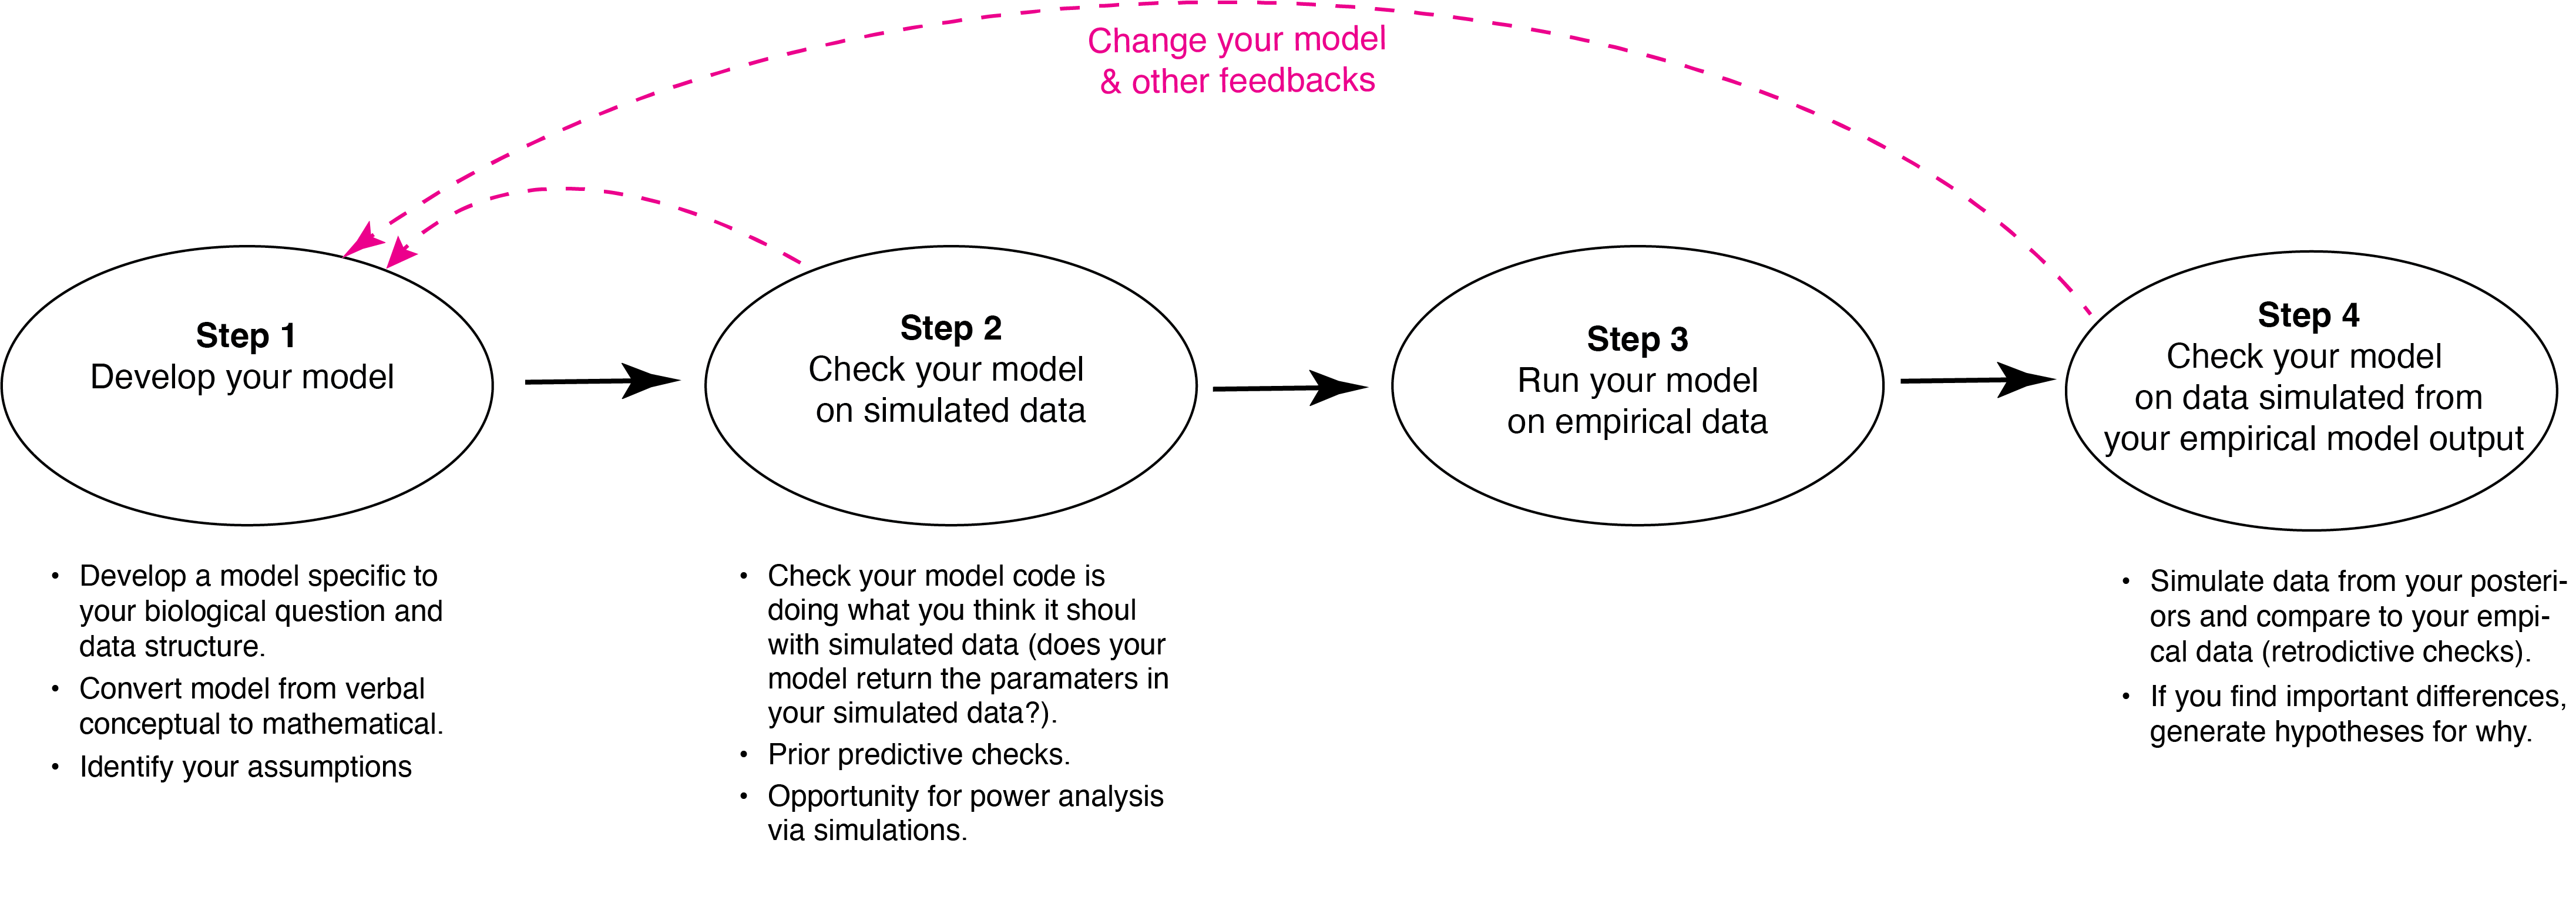
\includegraphics[width=1\textwidth]{..//figures/workflow.png}
\caption{The four-step iterative workflow we outline can help design models for specific ecological questions, data and aims---which makes this a statistical workflow that can naturally become a scientific workflow. It makes the step that many of us focus on---running your model on your empirical data (Step 3)---far more straightforward and insightful by using simulations both before (Step 2) and after (Step 4) it to better understand the model and data together.}
\label{fig:workflow}
\end{figure}

\begin{figure}[ht]
\centering
\noindent 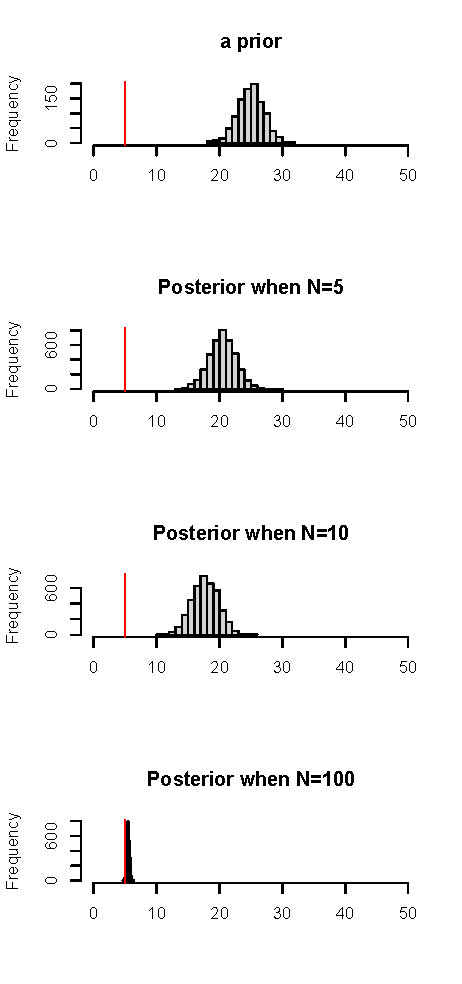
\includegraphics[width=0.5\textwidth]{..//examples/misspecifiedmodel/priorpostforflows.pdf}
\caption{A simple example of how to use simulated data to understand calibration issues in a mis-specified model. Here we know the true model underlying the data is $y=\alpha + \text{normal}(0, \sigma)$ where $\alpha$ is 5 (shown as blue vertical line) and $\sigma$ is 2. The model, however, is mis-specified by a prior for $\alpha$ of $\text{normal}(25, 2)$ (dashed blue line), resulting in a posterior (salmon-colored histogram) not centered on the true value. In our experience it is quite rare to have a prior informed by ecological knowledge be so far off, but this is an example. How mis-calibrated the model will be depends on the data: we show examples with a sample size ($N$) of 5, 10 and 40 data points. In practice these studies would allow us to determine how much data we would need to be robust to suspect prior models. (Note the change in $y$ axis range for bottom plot.) }
\label{fig:misspecifyprior}
\end{figure}

\end{document}

